\documentclass[12pt]{article}
\usepackage[papersize={8cm,12cm},margin={.5cm,.5cm}]{geometry}
\usepackage{common}
\begin{document}
\begin{problem}
  \item[1.] 數線上有 $O$、$A$、$B$ 三點,其中 $O$ 為原點,$A$ 點所表示的數為 $5 \times 10^2$,如圖(一)所示。根據圖(一)中數線上三點之間的實際距離進行估計,下列何者最接近 $B$ 點所表示的數?
  \begin{figure}[ht]
    \centering
    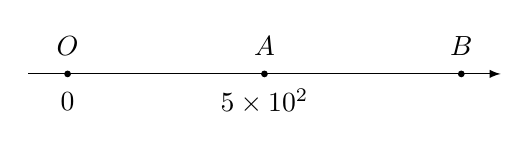
\begin{tikzpicture}
      \filldraw (.5,0) circle (1pt);
      \node at (.5,.35) {$O$};
      \node at (.5,-.35) {$0$};
      \filldraw (3,0) circle (1pt);
      \node at (3,.35) {$A$};
      \node at (3,-.35) {$5 \times 10^2$};
      \filldraw (5.5,0) circle (1pt);
      \node at (5.5,.35) {$B$};
      \draw[-latex] (0,0) -- (6,0);
    \end{tikzpicture}
    \caption*{圖(一)}
    \vspace*{-2ex}
  \end{figure}
  \begin{choices}
    \item $10^1$
    \item $10^2$
    \item $10^3$
    \item $10^4$
  \end{choices}
\end{problem}
\end{document}
